% !TEX root = ../ac_paper.tex

In this subsection we consider the size of neighborhoods of presentations.
A presentation is considered to be in the $k$-step neighborhood of another if they can be connected by applying at most $k$ AC moves.\footnote{For the experiments below we use the ``prime" AC moves as defined in \cref{?}. The results obtained using the classic AC moves are similar.}

In the previous subsections we explained how, using Proximal Policy Optimization, we labeled each of the presentations in the Miller–Schupp series for $n, \length(w) \leq 7$ as either ``solved" or ``unsolved," resulting in a total of 533 and 657 presentations respectively.
Our goal here is to analyze the relationship between these labels and the sizes of their respective 5-step neighborhoods.

There are 131 distinct neighborhood sizes in our data, their basic statistics are
\[
\begin{tabular}{cccccc}
	\toprule
	\textbf{Min} & \textbf{Max} & \textbf{Mean} & \textbf{Median} \\
	\midrule
	72,964 & 89,872 & 89,532 & 89,859 \\
	\bottomrule
\end{tabular}
\]
A more detailed description of the frequency of values is presented in \cref{fig:prime_combined_pie}.

\begin{figure}
	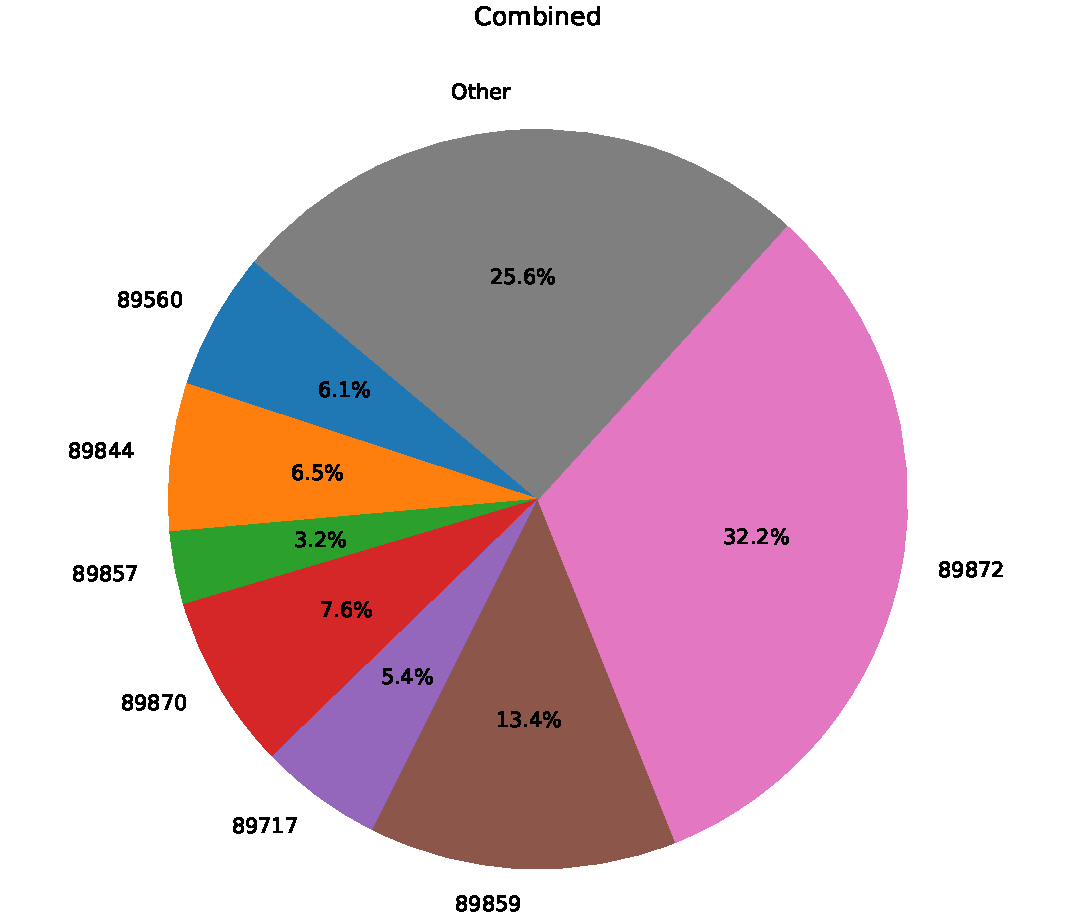
\includegraphics[scale=.4]{fig/prime_combined_pie_cropped.pdf}
	\caption{Sizes of the 5-step neighborhood of all considered presentations in the Miller–Schupp series. We group neighborhood sizes whose representation is below 2.5\%.}
	\label{fig:prime_combined_pie}
\end{figure}

The largest neighborhood size accounts for nearly a third of all considered presentations.
Yet, it represents only 7\% of solved presentations and more than half of the unsolved presentations.
Please consult \cref{fig:prime_pies} for more details.
Another notable feature visible in \cref{fig:prime_pies} is that only two neighborhood sizes account for almost three-quarters of all unsolved presentations.
Additionally, considering five sizes, this proportion reaches 94\%.
In fact, only ten neighborhood sizes are featured among unsolved presentations, whereas all 131 sizes appear among neighborhoods of solved presentations.
The most numerous neighborhood size for solved presentations is 89,560, accounting for only 13.5\% of these.
Furthermore, 41\% of all solved presentations have a neighborhood size that is shared by less than 2\% of solved presentations.

\begin{figure}
	\centering
	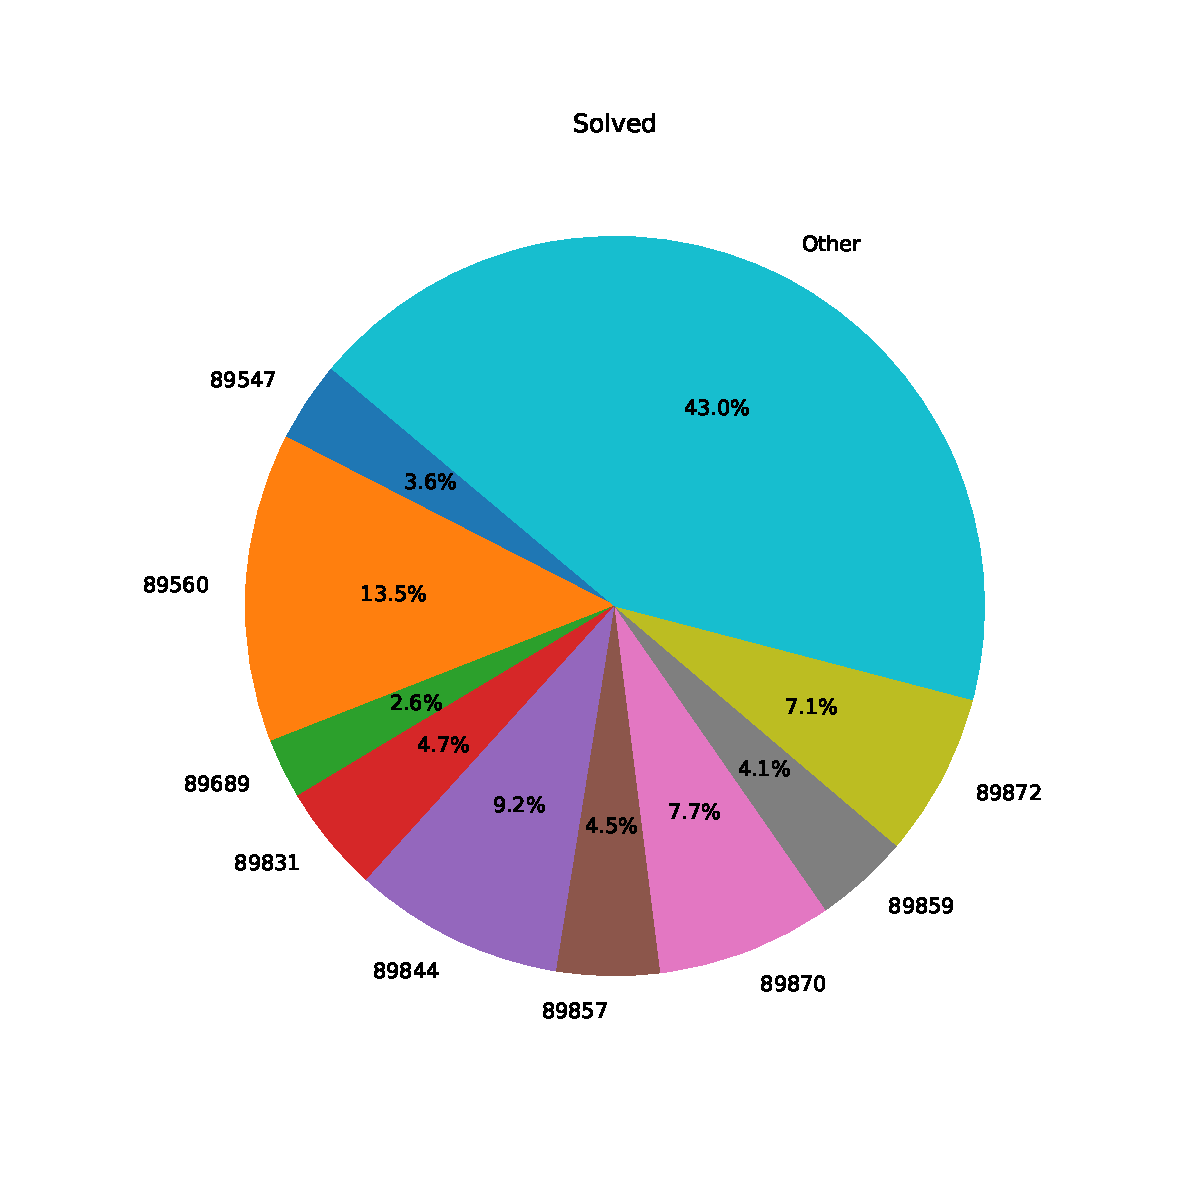
\includegraphics[scale=.4]{fig/prime_solved_pie_cropped.pdf}
	\quad
	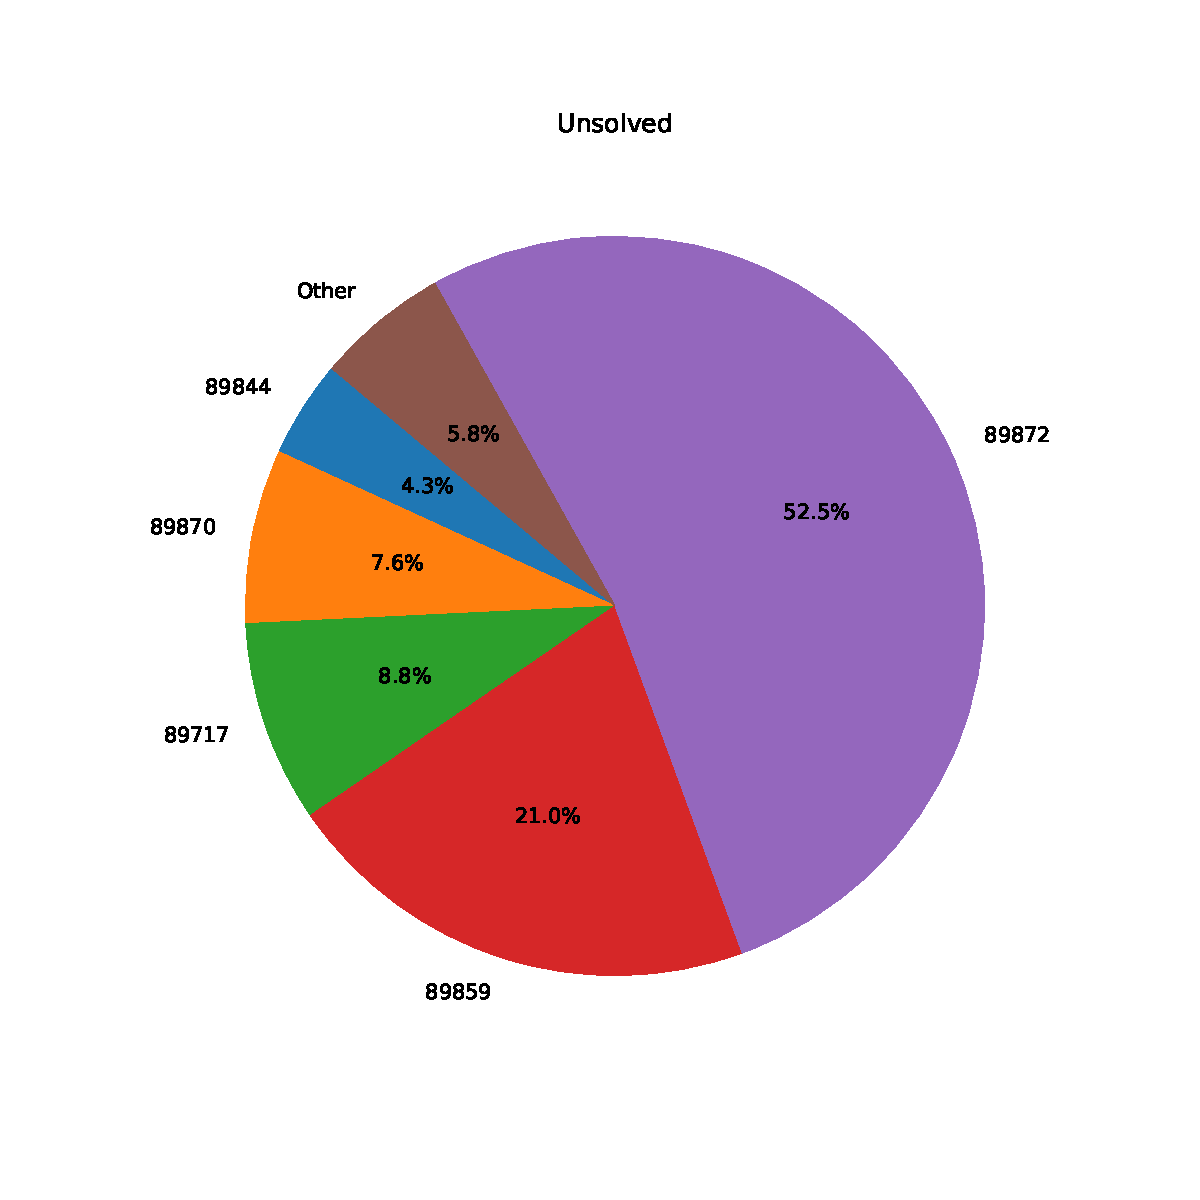
\includegraphics[scale=.4]{fig/prime_unsolved_pie_cropped.pdf}
	\caption{Pie charts for the neighborhood size of solved and unsolved presentations}
	\label{fig:prime_pies}
\end{figure}

%\begin{figure}[h!]
%	\centering
%	\begin{subfigure}[b]{0.45\textwidth}
%		\centering
%		\includegraphics[scale=.4]{fig/prime_solved_pie.pdf}
%	\end{subfigure}
%	\hfill
%	\begin{subfigure}[b]{0.45\textwidth}
%		\centering
%		\includegraphics[scale=.4]{fig/prime_unsolved_pie.pdf}
%	\end{subfigure}
%	\caption{Pie charts for the neighborhood size of solved and unsolved presentations}
%	\label{fig:prime_pies}
%\end{figure}

As we saw, having maximal neighborhood size provides significant information about the label of the presentation.
Additionally, the minimum neighborhood size among unsolved presentations --89,573-- is also quite informative since 42.2\% of solved presentations have neighborhood sizes less than that.
We can improve this percentage using that neighborhood sizes of unsolved presentations concentrate in three narrow bands. Please consult \cref{fig:prime_histogram}.
We have that 51\% of the solved presentations lie outside of the three bands $[89573, 89575]\ \& \ [89715, 89717]\ \& \ [89831, 89872]$ which contain 100\% of the unsolved presentations.
Let us replace the last band with $[89870, 89872]$.
In this case, the union of the three bands contain the neighborhood sizes of 93\% of unsolved presentations, whereas its complement contains 75\% of those associated to solved presentations.

\begin{figure}
	\centering
	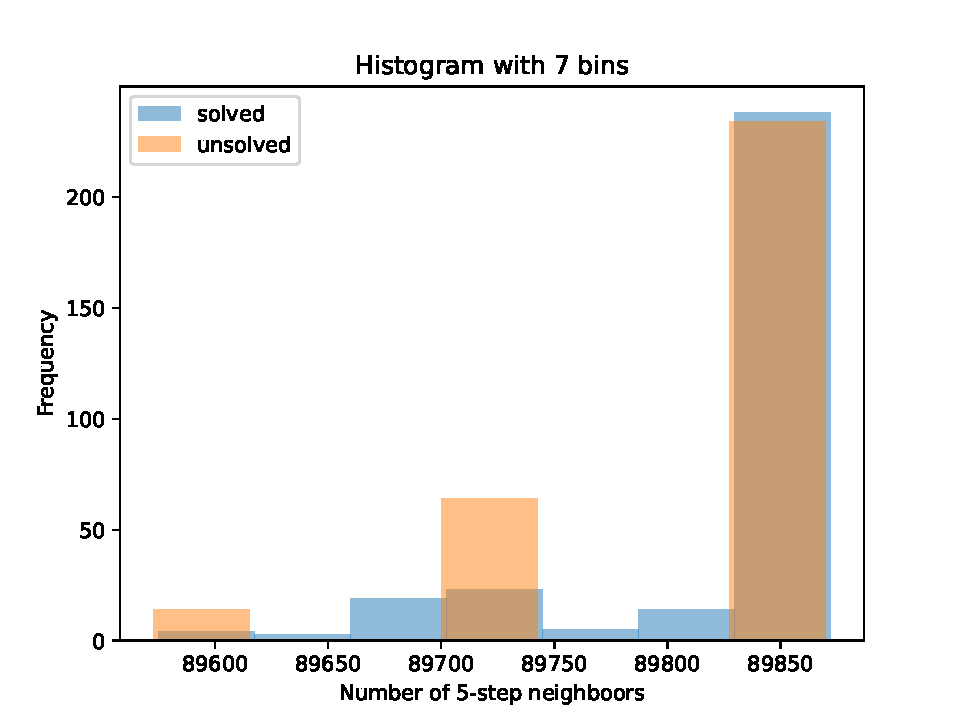
\includegraphics[scale=.34]{fig/prime_histogram.pdf}
	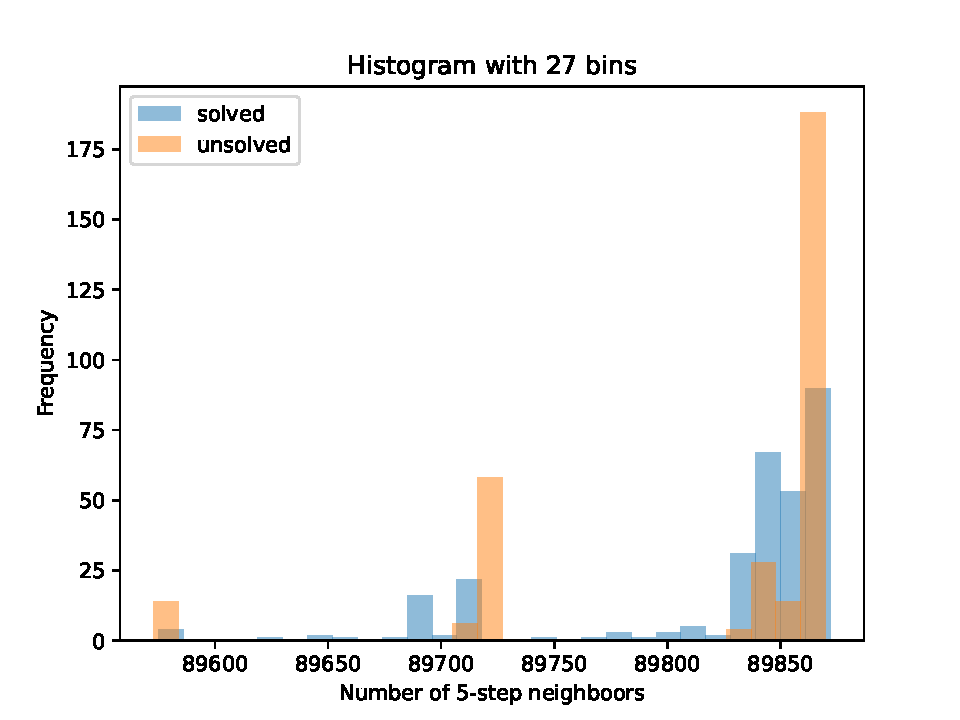
\includegraphics[scale=.34]{fig/prime_histogram2.pdf}
	\caption{Histograms with 7 and 27 bins respectively of the neighborhood sizes of the 533 solved and 657 unsolved presentations.}
	\label{fig:prime_histogram}
\end{figure}